\documentclass[aspectratio=169,11pt]{beamer}

\usetheme[progressbar=frametitle,numbering=fraction]{metropolis}

\usepackage[T1]{fontenc}
\usepackage{amsmath,amssymb}
\usepackage{array}
\usepackage{booktabs}
\usepackage{braket}
\usepackage{colortbl}
\usepackage{etoolbox}
\usepackage{fontawesome5}
\usepackage{microtype}
\usepackage{tabularx}
\usepackage{tikz}
\usepackage[
  backend=biber,
  style=alphabetic,
  maxalphanames=99,
  minalphanames=99,
  maxbibnames=99
]{biblatex}

\addbibresource{Quantum-Fair-Exchange/references.bib}
\renewcommand*{\multicitedelim}{\addcomma\space}

\usetikzlibrary{arrows.meta,calc,decorations.pathreplacing,fit,positioning}

% Speaker notes are embedded in the source but hidden in the normal deck.
% The small wrapper file used by `make notes` defines \showspeakernotes.
\ifdefined\showspeakernotes
  \setbeameroption{show notes on second screen=right}
  % pgfpages duplicates each logical page when composing the two-screen PDF;
  % disabling hyperlinks avoids duplicate PDF destinations in the notes copy.
  \hypersetup{draft}
\else
  \setbeameroption{hide notes}
\fi

% -----------------------------------------------------------------------------
% Visual language
% -----------------------------------------------------------------------------

\definecolor{QFEInk}{HTML}{17324D}
\definecolor{QFETeal}{HTML}{087E8B}
\definecolor{QFEPale}{HTML}{E8F3F4}
\definecolor{QFEGold}{HTML}{E5A23B}
\definecolor{QFEGoldPale}{HTML}{FFF2D8}
\definecolor{QFECoral}{HTML}{C85151}
\definecolor{QFECoralPale}{HTML}{F9E8E6}
\definecolor{QFEMuted}{HTML}{5E6D78}
\definecolor{QFEFog}{HTML}{F4F7F8}

\setbeamercolor{normal text}{fg=QFEInk,bg=white}
\setbeamercolor{alerted text}{fg=QFECoral}
\setbeamercolor{example text}{fg=QFETeal}
\setbeamercolor{frametitle}{fg=white,bg=QFEInk}
\setbeamercolor{progress bar}{fg=QFETeal,bg=QFEPale}
\setbeamercolor{progress bar in head/foot}{fg=QFETeal,bg=QFEPale}
\setbeamercolor{title separator}{fg=QFETeal}
\setbeamercolor{palette primary}{fg=white,bg=QFEInk}
\setbeamercolor{block title}{fg=white,bg=QFEInk}
\setbeamercolor{block body}{fg=QFEInk,bg=QFEFog}
\setbeamercolor{block title alerted}{fg=white,bg=QFECoral}
\setbeamercolor{block body alerted}{fg=QFEInk,bg=QFECoralPale}
\setbeamercolor{block title example}{fg=white,bg=QFETeal}
\setbeamercolor{block body example}{fg=QFEInk,bg=QFEPale}
\setbeamercolor{takeaway}{fg=QFEInk,bg=QFEPale}
\setbeamercolor{question}{fg=QFEInk,bg=QFEGoldPale}
\setbeamercolor{risk}{fg=QFEInk,bg=QFECoralPale}

\setbeamerfont{title}{series=\bfseries,size=\huge}
\setbeamerfont{subtitle}{size=\large}
\setbeamerfont{frametitle}{series=\bfseries,size=\Large}
\setbeamerfont{block title}{series=\bfseries}
\setbeamertemplate{navigation symbols}{}
\setbeamertemplate{bibliography item}[text]
\metroset{block=fill}

\newcommand{\asset}[1]{\ensuremath{\text{\$}_{#1}}}
\newcommand{\qasset}[1]{\ensuremath{\ket{\text{\$}_{#1}}}}
\newcommand{\qassetcopy}[2]{\ensuremath{\ket{\text{\$}_{#1}}^{(#2)}}}
\newcommand{\acclabel}{\ensuremath{\mathsf{Acc}}}
\newcommand{\rejlabel}{\ensuremath{\mathsf{Rej}}}
\newcommand{\badinput}[1]{\textcolor{QFECoral}{\textsf{#1}}}

\newcommand{\takeaway}[1]{%
  \begin{beamercolorbox}[wd=\textwidth,sep=0.85ex,rounded=true,center]{takeaway}
    #1
  \end{beamercolorbox}%
}

\newcommand{\questionbox}[1]{%
  \begin{beamercolorbox}[wd=\textwidth,sep=1.0ex,rounded=true,center]{question}
    #1
  \end{beamercolorbox}%
}

\newcommand{\riskbox}[2]{%
  \begin{beamercolorbox}[wd=\linewidth,sep=0.9ex,rounded=true]{risk}
    \textbf{#1}\par\smallskip
    \small #2
  \end{beamercolorbox}%
}

% One fixed-coordinate diagram is reused for all four functionality slides.
% Arguments: Alice input, Bob input, Alice output, Bob output. Empty output
% arguments suppress the corresponding arrow while preserving the bounding box.
\newcommand{\exchangefunctionality}[4]{%
  \begin{tikzpicture}[
      >={Latex[length=2.6mm]},
      flow/.style={->,very thick,draw=QFETeal},
      party/.style={font=\large\bfseries,text=QFEInk},
      arrowlabel/.style={font=\large,fill=white,inner sep=2pt},
      function/.style={draw=QFEInk,fill=QFEInk,rounded corners=4pt,
        minimum width=3.35cm,minimum height=3.05cm,align=center,
        text=white,font=\large\bfseries}
    ]
    \path[use as bounding box] (-5.15,-2.10) rectangle (5.15,2.10);

    \node[party] at (-4.15,1.60) {Alice};
    \node[party] at ( 4.15,1.60) {Bob};
    \node[function] (fe) at (0,0) {Fair\\Exchange};

    \draw[flow] (-4.75,0.62) --
      node[arrowlabel,above] {#1} ([yshift=0.62cm]fe.west);
    \draw[flow] (4.75,0.62) --
      node[arrowlabel,above] {#2} ([yshift=0.62cm]fe.east);

    \ifstrempty{#3}{}{
      \draw[flow] ([yshift=-0.62cm]fe.west) --
        node[arrowlabel,below] {#3} (-4.75,-0.62);
    }
    \ifstrempty{#4}{}{
      \draw[flow] ([yshift=-0.62cm]fe.east) --
        node[arrowlabel,below] {#4} (4.75,-0.62);
    }
  \end{tikzpicture}%
}

% -----------------------------------------------------------------------------
% Metadata (sourced from the technical manuscript in the submodule)
% -----------------------------------------------------------------------------

\title{Quantum Fair Exchange}
\subtitle{How do we exchange a state that cannot be copied?}
\author[Chung, Lee, Raizes, Thyagarajan]{%
  \texorpdfstring{%
    Hao Chung \quad Yi Lee \quad Justin Raizes\\[0.15em]
    Sri AravindaKrishnan Thyagarajan%
  }{Hao Chung, Yi Lee, Justin Raizes, Sri AravindaKrishnan Thyagarajan}}
\institute{%
  LayerZero Labs \;\textperiodcentered\; University of Maryland\\
  NTT Research \;\textperiodcentered\; University of Sydney}
\date{Ongoing work}

\begin{document}

% -----------------------------------------------------------------------------
% 1. Title
% -----------------------------------------------------------------------------

\begin{frame}[plain]
  \vfill
  {\usebeamerfont{title}\color{QFEInk}\inserttitle\par}
  \vspace{0.4em}
  {\usebeamerfont{subtitle}\color{QFEMuted}\insertsubtitle\par}
  \vspace{0.8em}
  {\color{QFETeal}\rule{0.48\textwidth}{1.2pt}\par}

  \vspace{1.2em}
  {\small\bfseries\insertauthor\par}
  \vspace{0.65em}
  {\footnotesize\color{QFEMuted}\insertinstitute\par}

  \vfill
  {\footnotesize\bfseries\color{QFEGold}\insertdate\par}
\end{frame}

% -----------------------------------------------------------------------------
% 2. Motivation
% -----------------------------------------------------------------------------

\begin{frame}{Fair Exchange: Who Goes First?}
  \begin{center}
    \begin{tikzpicture}[
        >={Latex[length=3mm]},
        party/.style={draw=QFEInk,fill=QFEFog,circle,minimum size=1.55cm,
          very thick,font=\bfseries},
        trade/.style={<->,line width=1.5pt,draw=QFETeal}
      ]
      \node[party] (alice) at (-4.2,0) {Alice};
      \node[party] (bob) at (4.2,0) {Bob};
      \draw[trade] (alice) -- (bob)
        node[pos=0.35,above=5pt,font=\large\bfseries,text=QFEInk]
          {\faMoneyBill\; \$100}
        node[pos=0.67,below=5pt,font=\large\bfseries,text=QFEInk]
          {\faIcon{ticket-alt}\; Digital ticket};
      \node[font=\Large\bfseries,text=QFEGold] at (0,1.28) {Who goes first?};
    \end{tikzpicture}
  \end{center}

  \begin{columns}[T,onlytextwidth]
    \column{0.485\textwidth}
      \riskbox{If Alice pays first\ldots}{Bob can take the money and disappear.}
    \column{0.485\textwidth}
      \riskbox{If Bob sends first\ldots}{Alice can take the ticket and disappear.}
  \end{columns}

  \vspace{0.55em}
  \takeaway{\textbf{Goal:} Either both get what they want, or neither does.}

  \note{
    \begin{itemize}
      \item Start from the intuitive problem, before introducing cryptographic definitions.
      \item ``Digital ticket'' can mean a concert ticket, game activation or serial code, or gift-card code.
      \item Alice and Bob do not necessarily trust each other; either may cheat.
      \item Pause at ``Who goes first?'' before explaining the two cheating cases.
      \item Keep this slide mostly visual and light on text.
    \end{itemize}
  }
\end{frame}

% -----------------------------------------------------------------------------
% 3. Trusted intermediary
% -----------------------------------------------------------------------------

\begin{frame}{The Obvious Solution: A Trusted Third Party}
  \centering
    \begin{tikzpicture}[
        >={Latex[length=2.7mm]},
        party/.style={draw=QFEInk,fill=QFEFog,circle,minimum size=1.18cm,
          very thick,font=\bfseries},
        bank/.style={draw=QFEInk,fill=QFEGoldPale,rounded corners=3pt,
          minimum width=3.1cm,minimum height=0.75cm,very thick,font=\bfseries},
        payment/.style={->,very thick,draw=QFEGold},
        ticket/.style={->,very thick,draw=QFETeal}
      ]
      \node[party] (alice) at (-4.4,-0.72) {Alice};
      \node[party] (bob) at (4.4,-0.72) {Bob};
      \node[bank] (bank) at (0,0.92) {\faUniversity\quad Bank / card network};

      \draw[payment] (alice.north east) --
        node[above left=-1pt,font=\small\bfseries,text=QFEGold!70!black] {\$100}
        (bank.south west);
      \draw[payment] (bank.south east) --
        node[above right=-1pt,font=\small\bfseries,text=QFEGold!70!black] {payment}
        (bob.north west);
      \draw[ticket] (bob.west) --
        node[below=4pt,font=\small\bfseries,text=QFETeal] {\faIcon{ticket-alt}\quad Digital ticket (direct)}
        (alice.east);
    \end{tikzpicture}

  \vspace{0.15em}
  \begin{columns}[T,onlytextwidth]
    \column{0.48\textwidth}
      \begin{block}{Trusted institutions can intervene}
        \small Credit-card disputes and chargebacks; online marketplaces.
      \end{block}
    \column{0.48\textwidth}
      \begin{alertblock}{Cash-like exchange?}
        \small Can Alice and Bob exchange directly?
      \end{alertblock}
  \end{columns}

  \vspace{-0.1em}
  \scriptsize \textbf{Cryptocurrency:} direct transactions need not use a trusted
  intermediary. \quad \textbf{Later:} quantum money as digital cash.

  \vspace{0.3em}
  \takeaway{\textbf{Fair exchange matters when Alice and Bob transact directly.}}

  \note{
    \footnotesize
    \begin{itemize}
      \item The obvious real-world solution is to trust someone else.
      \item With a credit card, a trusted institution can intervene through a dispute or chargeback mechanism.
      \item Do not dwell on the exact mechanics of the ticket example.
      \item Contrast this with physical cash: the central bank does not participate in a particular hand-to-hand transaction.
      \item This motivates digital value that can transfer without a trusted intermediary approving every transaction.
      \item Cryptocurrency is the familiar example; do not claim it has no trusted parties at all.
      \item Preview quantum money here and explain it on the next slide.
      \item The ticket travels directly from Bob to Alice; only the payment path uses the trusted institution.
    \end{itemize}
  }
\end{frame}

% -----------------------------------------------------------------------------
% 4. Two kinds of digital cash
% -----------------------------------------------------------------------------

\begin{frame}{Digital Cash: Blockchain vs. Quantum Money}
  \small
  \renewcommand{\arraystretch}{1.45}
  \setlength{\tabcolsep}{6pt}
  \begin{tabularx}{\textwidth}{%
      >{\raggedright\arraybackslash\bfseries}p{0.18\textwidth}
      >{\raggedright\arraybackslash}X
      >{\raggedright\arraybackslash}X}
    \toprule
    & \textbf{Cryptocurrency / Blockchain} & \textbf{Quantum Money} \\
    \midrule
    Issuance & Mining / protocol & Bank / issuer \\
    Prevent double spending & Global ledger / consensus & No-cloning + cryptography \\
    Transfer & Record the transfer on a global blockchain & Send the quantum state \\
    \rowcolor{QFEGoldPale}
    Fair exchange & Atomic swaps / smart contracts &
      \centering\arraybackslash\textcolor{QFEGold}{\Large\bfseries ???} \\
    \bottomrule
  \end{tabularx}

  \vspace{0.85em}
  \takeaway{\faMoneyBill\quad \textbf{Quantum money behaves more like a digital banknote.}}

  \note{
    \begin{itemize}
      \item Cryptocurrency and quantum money are two very different approaches to digital cash.
      \item For cryptocurrency, issuance can be governed by mining or a protocol; for quantum money, imagine a bank minting quantum banknotes.
      \item The key contrast is transfer: a blockchain records it globally, whereas quantum money transfers the state itself.
      \item The bank may mint quantum money without mediating every payment.
      \item Atomic swaps and smart contracts can implement fair exchange for blockchain-based assets.
      \item Pause at the final ``???'' and ask for the analogue for quantum money.
      \item No-cloning alone is not a construction of secure quantum money; this table is deliberately simplified.
    \end{itemize}
  }
\end{frame}

% -----------------------------------------------------------------------------
% 5--8. The functionality sequence
% -----------------------------------------------------------------------------

\begin{frame}{Classical Fair Exchange}
  \centering
  \exchangefunctionality{\asset{A}}{\asset{B}}{\asset{B}}{\asset{A}}

  \vspace{0.2em}
  {\large If both inputs are valid, \textbf{swap them}.\par}

  \note{
    \begin{itemize}
      \item Abstract away the implementation and imagine an ideal fair-exchange box.
      \item Alice submits her classical asset \asset{A}; Bob submits \asset{B}.
      \item If both inputs are valid, the functionality swaps them.
      \item Keep this slide simple; cheating and rejection come next.
    \end{itemize}
  }
\end{frame}

\begin{frame}{Classical Fair Exchange: Rejection}
  \centering
  \exchangefunctionality{\asset{A}}{\badinput{garbage}}{\textcolor{QFECoral}{\rejlabel}}{}

  \vspace{0.2em}
  {\large If Bob submits an invalid asset, Alice receives \textbf{\rejlabel}.\par}

  \note{
    \begin{itemize}
      \item Bob may cheat and submit garbage instead of a valid asset.
      \item The ideal functionality rejects and tells Alice \rejlabel.
      \item There is no need to return \asset{A}: this is classical information, so Alice can already retain or know her input.
      \item This apparently trivial point becomes important when the asset is quantum.
    \end{itemize}
  }
\end{frame}

\begin{frame}{Quantum Fair Exchange: Rejection?}
  \centering
  \exchangefunctionality{\qasset{A}}{\badinput{garbage}}{\textcolor{QFECoral}{\rejlabel}}{}

  \vspace{0.2em}
  {\LARGE\bfseries\color{QFEGold}Where is Alice's money?\par}

  \note{
    \begin{itemize}
      \item Change only one thing from the previous slide: Alice's asset is now a quantum state.
      \item Classically, returning only \rejlabel{} was fine because Alice could retain her input.
      \item Alice may have sent her only copy of \qasset{A} into the protocol.
      \item If Bob cheats and the protocol simply rejects, Alice may have lost her asset.
      \item Pause on ``Where is Alice's money?''
      \item This is why the classical ideal functionality is no longer the right notion.
    \end{itemize}
  }
\end{frame}

\begin{frame}{Quantum Fair Exchange: Rejection}
  \centering
  \exchangefunctionality{\qasset{A}}{\badinput{garbage}}{\qasset{A}\; +\; \textcolor{QFECoral}{\rejlabel}}{}

  \vspace{0.2em}
  {\large If Bob submits an invalid asset, Alice gets her
    \textbf{quantum asset back}.\par}

  \note{
    \begin{itemize}
      \item Rejection must preserve the honest party's asset.
      \item If Bob cheats, Alice should recover a usable quantum asset, not merely learn that the exchange failed.
      \item This is nontrivial because Alice cannot generally keep a backup copy of an unknown quantum state.
      \item This is the key change in the ideal functionality caused by no-cloning.
      \item Next, formalize what counts as a valid or usable returned asset, especially when verification can transform the state.
    \end{itemize}
  }
\end{frame}

% -----------------------------------------------------------------------------
% 9. Related work
% -----------------------------------------------------------------------------

\begin{frame}{Literature Survey}
  \begin{columns}[T,onlytextwidth]
    \column{0.31\textwidth}
      \begin{block}{Classical fair exchange}
        \small
        Studied since the early 1980s.

        \medskip
        Contract signing, trusted third parties, and a long line of related work.
      \end{block}

    \column{0.335\textwidth}
      \begin{block}{MPQC with identifiable abort}
        \small
        Identify the cheating party and abort.

        \medskip
        \cite{alon-et-al-identifiable-abort,chung-et-al-pvia}
      \end{block}

    \column{0.31\textwidth}
      \begin{block}{Verifiable QFHE}
        \small
        A key technical building block.

        \medskip
        \cite{alagic-et-al-vqfhe}
      \end{block}
  \end{columns}

  \vspace{0.9em}
  \questionbox{\textbf{Accountability is not restitution:}
    identifying a cheater does not restore a lost quantum asset.}

  \note{
    \begin{itemize}
      \item Keep the classical literature deliberately brief; it dates to the early 1980s.
      \item If useful: ``Aravind probably knows much more of this history than I do, so I'll skip ahead about forty years.''
      \item The closest quantum line here is multiparty quantum computation with identifiable abort.
      \item Identifiable abort gives accountability: identify the cheating party and abort.
      \item Fair exchange also asks what happens to the honest party's quantum asset.
      \item Mention VQFHE only as a technical building block; review it later.
    \end{itemize}
  }
\end{frame}

% -----------------------------------------------------------------------------
% 10. Main goals
% -----------------------------------------------------------------------------

\begin{frame}{Main Goals}
  \small
  We propose an ideal functionality for \textbf{quantum fair exchange}, adapting
  classical fair exchange to the limitations imposed by quantum no-cloning.

  \smallskip
  \textbf{We aim to show two complementary results:}

  \smallskip
  \begin{columns}[T,onlytextwidth]
    \column{0.475\textwidth}
      \begin{alertblock}{1\quad Classical TTP: impossible in general}
        Quantum fair exchange is impossible in general, even with a
        \textbf{classical trusted third party}.
      \end{alertblock}

    \column{0.475\textwidth}
      \begin{exampleblock}{2\quad Limited quantum capabilities suffice}
        A trusted party may use \textbf{quantum pre-processing and storage}.

        \smallskip
        Online, it performs no quantum computation other than \textbf{SWAP gates}.
      \end{exampleblock}
  \end{columns}

  \vspace{-0.1em}
  \takeaway{Finally, extend the construction to \textbf{$n$-party exchange}.}

  \note{
    \begin{itemize}
      \item These are goals and ongoing results, so say ``we aim to show,'' not ``we prove.''
      \item Emphasize the complementarity: a fully classical trusted party is insufficient, but surprisingly limited quantum capabilities suffice.
      \item The resource question is not simply whether a trusted party exists, but which quantum capabilities it needs.
      \item Do not explain the technical reason yet; begin the next section with the impossibility result and its intuition.
      \item Mention the $n$-party extension briefly; it need not have equal visual weight.
    \end{itemize}
  }
\end{frame}

% -----------------------------------------------------------------------------
% 11--14. Impossibility via a direct cloning reduction
% -----------------------------------------------------------------------------

\begin{frame}{Impossibility with a Classical Trusted Party}
  \centering
  {\large Assume a $T$-round fair-exchange protocol $\Pi$ with a
    \textbf{classical TTP}.\par}

  \vspace{0.55em}
  {\Large
  \(
    \bigl(\qasset{A},\qasset{B}\bigr)
      \xrightarrow{\quad\Pi\quad}
    \bigl(\qasset{B},\qasset{A}\bigr)
  \)\par}

  \vspace{0.45em}
  {\small Success swaps the assets; abort restores the honest party's own
    asset.\par}

  \vspace{0.55em}
  \begin{alertblock}{$\Pi$ becomes a cloning procedure}
    \centering
    \Large
    $\Pr[\text{duplicate one input}]
      =\Omega\!\left(\dfrac{1}{T}\right).$
  \end{alertblock}

  \vspace{0.15em}
  {\normalsize\bfseries One identified asset
    $\not\longmapsto$ two usable copies.\par}

  \note{
    \footnotesize
    \begin{itemize}
      \item Hard-code perfect honest correctness for the talk: $p=1$. The general statement replaces $1/(2T)$ by $p/(2T)$, up to fairness and correctness errors.
      \item The $1/T$ quantity is the cloning attack's success scale, not an upper bound on honest protocol success.
      \item Operational unclonability means that, from one identified asset, producing two usable versions of that same asset has negligible probability.
      \item Textbook deterministic no-cloning alone is not a quantitative security game. BB84 is one concrete witness used by the longer manuscript proof; omit it here.
      \item Alice and Bob may exchange quantum messages. Only the trusted party is restricted to copyable classical state.
      \item Keep the statement informal while the complete model and error parameters are still being finalized.
    \end{itemize}
  }
\end{frame}

\begin{frame}{Somewhere, the Exchange Must Happen}
  \centering
  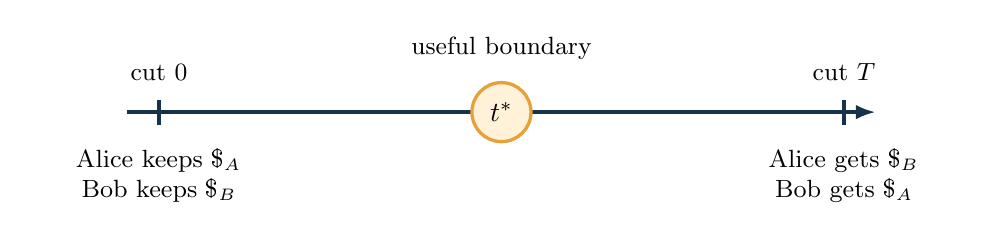
\begin{tikzpicture}[
      >={Latex[length=2.5mm]},
      timeline/.style={->,very thick,draw=QFEInk},
      tick/.style={very thick,draw=QFEInk},
      endpoint/.style={align=center,font=\small},
      pivotal/.style={draw=QFEGold,fill=QFEGoldPale,circle,minimum size=0.75cm,
        very thick,font=\bfseries}
    ]
    \draw[timeline] (-4.75,0) -- (4.75,0);
    \draw[tick] (-4.35,0.16) -- (-4.35,-0.16);
    \draw[tick] (4.35,0.16) -- (4.35,-0.16);
    \node[pivotal] at (0,0) {$t^*$};

    \node[endpoint,anchor=south] at (-4.35,0.28) {cut $0$};
    \node[endpoint,anchor=south] at (0,0.55) {useful boundary};
    \node[endpoint,anchor=south] at (4.35,0.28) {cut $T$};

    \node[endpoint,anchor=north,text width=3.1cm] at (-4.35,-0.34)
      {Alice keeps \asset{A}\\Bob keeps \asset{B}};
    \node[endpoint,anchor=north,text width=3.1cm] at (4.35,-0.34)
      {Alice gets \asset{B}\\Bob gets \asset{A}};
  \end{tikzpicture}

  \vspace{0.6em}
  {\large Some neighboring pair of cuts must witness the handoff.\par}

  \vspace{0.55em}
  \takeaway{With $T$ possible boundaries, the reduction loses one factor of
    $T$.}

  \note{
    \footnotesize
    \begin{itemize}
      \item This slide is deliberately operational. Do not define cut-acceptance probabilities.
      \item Initially, stopping leaves each party with its own asset. At honest completion, the assets have swapped.
      \item In the formal proof, if the parties already disagree at one cut, use that cut. Otherwise some party's outcome changes across neighboring cuts.
      \item One of the $T$ locations is therefore useful. The reduction can hardwire it; the random-guess cartoon explains the $1/T$ scale.
      \item The next two slides show what the reduction does at that location.
    \end{itemize}
  }
\end{frame}

\begin{frame}{Reduction: Fork the Classical World}
  \begin{columns}[T,onlytextwidth]
    \column{0.45\textwidth}
      \centering
      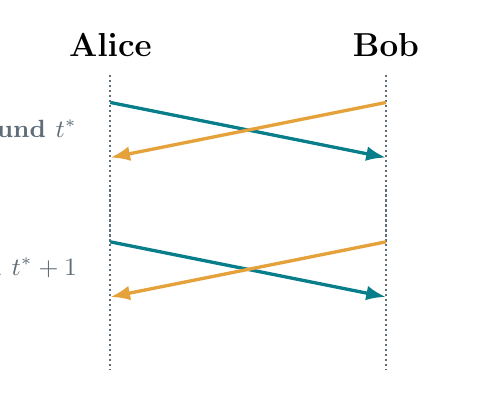
\begin{tikzpicture}[
          >={Latex[length=2.5mm]},
          lane/.style={densely dotted,thick,draw=QFEMuted},
          amsg/.style={->,very thick,draw=QFETeal},
          bmsg/.style={->,very thick,draw=QFEGold},
          party/.style={font=\large\bfseries},
          round/.style={font=\small\bfseries,text=QFEMuted}
        ]
        \path[use as bounding box] (-2.8,-2.40) rectangle (2.8,2.0);
        \node[party] (alice) at (-1.75,1.78) {Alice};
        \node[party] (bob) at (1.75,1.78) {Bob};
        \draw[lane] (-1.75,1.4) -- (-1.75,-2.35);
        \draw[lane] (1.75,1.4) -- (1.75,-2.35);

        \node[round,anchor=east] at (-2.05,0.72) {round $t^*$};
        \draw[amsg] (-1.75,1.05) -- (1.75,0.35);
        \draw[bmsg] (1.75,1.05) -- (-1.75,0.35);

        \node[round,anchor=east] at (-2.05,-1.05) {round $t^*+1$};
        \draw[amsg] (-1.75,-0.72) -- (1.75,-1.42);
        \draw[bmsg] (1.75,-0.72) -- (-1.75,-1.42);

      \end{tikzpicture}

    \column{0.52\textwidth}
      \vspace{0.25em}
      {\large\bfseries 1\quad Run the honest prefix.\par}

      \vspace{0.55em}
      {\large The referee holds a classical state $c_{t^*}$.\par}

      \vspace{0.55em}
      \begin{center}
        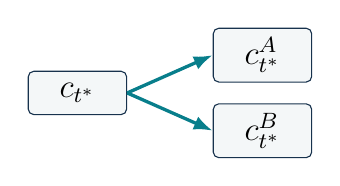
\begin{tikzpicture}[
            >={Latex[length=2.4mm]},
            state/.style={draw=QFEInk,fill=QFEFog,rounded corners=2pt,
              minimum width=1.25cm,minimum height=0.55cm,font=\large},
            fork/.style={->,very thick,draw=QFETeal}
          ]
          \node[state] (c) at (0,0) {$c_{t^*}$};
          \node[state] (ca) at (2.35,0.48) {$c_{t^*}^{A}$};
          \node[state] (cb) at (2.35,-0.48) {$c_{t^*}^{B}$};
          \draw[fork] (c.east) -- (ca.west);
          \draw[fork] (c.east) -- (cb.west);
        \end{tikzpicture}
      \end{center}

      \vspace{0.55em}
      {\large\bfseries 2\quad Form two locally consistent continuations.\par}
  \end{columns}

  \vspace{0.2em}
  \takeaway{Only the \textbf{classical referee state} is copied---not either
    quantum asset.}

  \note{
    \footnotesize
    \begin{itemize}
      \item Run the honest protocol up to the useful boundary on the two challenge assets.
      \item The reduction simulates the trusted party. Because its complete state is classical, the reduction can copy it exactly.
      \item Alice and Bob are then continued against different copies of the referee state. Each continuation is locally consistent with the honest prefix.
      \item The intact arrows indicate the neighboring-round alternatives used by the proof; do not analyze their probabilities on the slide.
      \item This classical fork is precisely what becomes unavailable when the trusted party holds quantum state.
    \end{itemize}
  }
\end{frame}

\begin{frame}{Reduction: Let One Message Through}
  \begin{columns}[T,onlytextwidth]
    \column{0.47\textwidth}
      \centering
      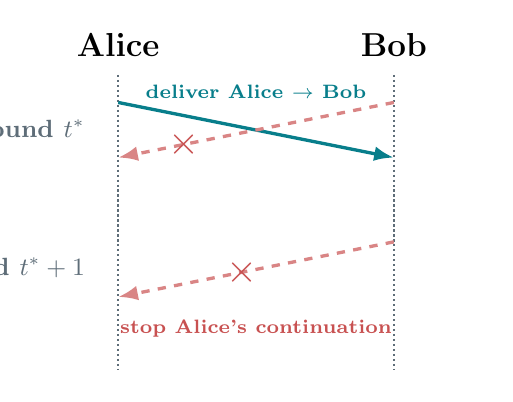
\begin{tikzpicture}[
          >={Latex[length=2.5mm]},
          lane/.style={densely dotted,thick,draw=QFEMuted},
          delivered/.style={->,very thick,draw=QFETeal},
          blocked/.style={->,very thick,dashed,draw=QFECoral!70},
          party/.style={font=\large\bfseries},
          round/.style={font=\small\bfseries,text=QFEMuted}
        ]
        \path[use as bounding box] (-2.9,-2.40) rectangle (2.9,2.0);
        \node[party] at (-1.75,1.78) {Alice};
        \node[party] at (1.75,1.78) {Bob};
        \draw[lane] (-1.75,1.4) -- (-1.75,-2.35);
        \draw[lane] (1.75,1.4) -- (1.75,-2.35);

        \node[round,anchor=east] at (-2.05,0.72) {round $t^*$};
        \draw[delivered] (-1.75,1.05) -- (1.75,0.35);
        \draw[blocked] (1.75,1.05) --
          node[pos=0.76,font=\Large,text=QFECoral] {$\times$}
          (-1.75,0.35);

        \node[round,anchor=east] at (-2.05,-1.05) {round $t^*+1$};
        \draw[blocked] (1.75,-0.72) --
          node[pos=0.55,font=\Large,text=QFECoral] {$\times$}
          (-1.75,-1.42);
        \node[font=\scriptsize\bfseries,text=QFETeal] at (0,1.18)
          {deliver Alice $\to$ Bob};
        \node[font=\scriptsize\bfseries,text=QFECoral] at (0,-1.82)
          {stop Alice's continuation};
      \end{tikzpicture}

    \column{0.50\textwidth}
      \centering
      \vspace{0.45em}
      {\large\bfseries Alice's continuation $c_{t^*}^{A}$\par}
      \smallskip
      Bob stopped

      \smallskip
      {\Large $\rejlabel\; +\; \qassetcopy{A}{A}$\par}

      \vspace{0.65em}
      {\color{QFEMuted}\rule{0.70\linewidth}{0.5pt}\par}
      \vspace{0.55em}

      {\large\bfseries Bob's continuation $c_{t^*}^{B}$\par}
      \smallskip
      Alice's message arrived

      \smallskip
      {\Large $\acclabel\; +\; \qassetcopy{A}{B}$\par}
  \end{columns}

  \vspace{0em}
  \questionbox{\qassetcopy{A}{A}\qquad \qassetcopy{A}{B}\qquad
    \textbf{two usable copies from one input}.}

  \note{
    \footnotesize
    \begin{itemize}
      \item Alice and Bob continue against different copies of the classical trusted-party state.
      \item In the orientation drawn, Bob has crossed the pivotal boundary and Alice has not.
      \item If Bob accepts, he must hold Alice's original asset. If Alice rejects, asset-preserving abort must restore that same input to her.
      \item The two outputs must be versions of the same identified asset, or pass the same instance-specific verifier; merely passing a broad type verifier is not enough.
      \item If the flags are reversed, the reduction duplicates Bob's input instead.
      \item If the rejecting party receives nothing, fairness has already failed.
      \item The full proof has simultaneous-cut and staggered-cut cases. The removed stopping-probability analysis establishes that one of the $T$ locations works with the claimed $1/T$ scale.
      \item Transition: quantum custody prevents this classical fork, pointing toward the positive construction.
    \end{itemize}
  }
\end{frame}

% -----------------------------------------------------------------------------
% 15--20. Six one-idea preliminaries
% -----------------------------------------------------------------------------

\begin{frame}{QEC: Spread One Qubit Across a Block}
  \centering
  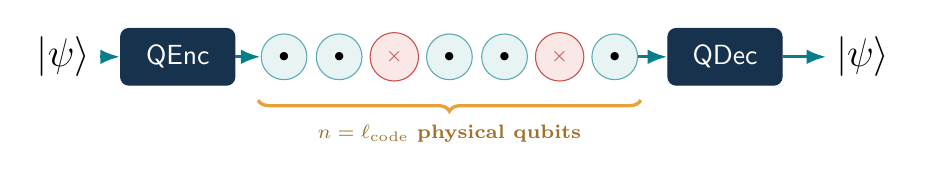
\begin{tikzpicture}[
      >={Latex[length=2.5mm]},
      flow/.style={->,very thick,draw=QFETeal},
      process/.style={draw=QFEInk,fill=QFEInk,rounded corners=3pt,
        text=white,minimum width=1.45cm,minimum height=0.72cm,font=\bfseries},
      qubit/.style={draw=QFETeal!65,fill=QFEPale,circle,
        minimum size=0.58cm,font=\scriptsize\bfseries}
    ]
    \node[font=\Large] (in) at (-5.15,0.65) {$\ket\psi$};
    \node[process] (enc) at (-3.70,0.65) {$\mathsf{QEnc}$};
    \draw[flow] (in) -- (enc);

    \foreach \x/\name in {-2.35/q1,-1.65/q2,-0.95/q3,-0.25/q4,0.45/q5,1.15/q6,1.85/q7} {
      \node[qubit] (\name) at (\x,0.65) {$\bullet$};
    }
    \draw[flow] (enc) -- (q1);
    \node[qubit,draw=QFECoral,fill=QFECoralPale,text=QFECoral] at (-0.95,0.65) {$\times$};
    \node[qubit,draw=QFECoral,fill=QFECoralPale,text=QFECoral] at (1.15,0.65) {$\times$};

    \node[process] (dec) at (3.25,0.65) {$\mathsf{QDec}$};
    \node[font=\Large] (out) at (5.00,0.65) {$\ket\psi$};
    \draw[flow] (q7) -- (dec);
    \draw[flow] (dec) -- (out);

    \draw[decorate,decoration={brace,mirror,amplitude=4pt},very thick,draw=QFEGold]
      (-2.68,0.10) -- (2.18,0.10)
      node[midway,below=5pt,font=\scriptsize\bfseries,text=QFEGold!70!black]
      {$n=\ell_{\mathrm{code}}$ physical qubits};
  \end{tikzpicture}

  \vspace{0.6em}
  {\small\bfseries One entangled block---not $n$ copies of $\ket\psi$.\par}

  \vspace{0.5em}
  \begin{exampleblock}{Correct up to $r$ damaged positions per block}
    \centering
    $\displaystyle
      \mathsf{QDec}\!\left(E\,\mathsf{QEnc}(\rho)E^\dagger\right)=\rho
      \quad\text{when}\quad
      \mathsf{wt}(E)\leq r=\left\lfloor\frac{d_{\mathrm{code}}-1}{2}\right\rfloor.$
  \end{exampleblock}

  \vspace{-0.2em}
  \takeaway{Quantum error correction makes \textbf{bounded damage repairable}.}

  \note{
    \footnotesize
    \begin{itemize}
      \item Keep this at the one-idea level: encode one logical qubit into an entangled block of $n$ physical qubits.
      \item Emphasize that this is not cloning. No individual physical qubit contains a copy of the unknown input.
      \item The manuscript uses an $[[\ell_{\mathrm{code}},1,d_{\mathrm{code}}]]$ code and corrects errors of weight at most $\lfloor(d_{\mathrm{code}}-1)/2\rfloor$ per block.
      \item Authentication will detect adversarial tampering; QEC repairs the bounded residual damage.
    \end{itemize}
  }
\end{frame}

\begin{frame}{Transversal Operations: Compute Coordinatewise}
  \centering
  {\Large\bfseries Example: \quad $X_L=X^{\otimes n}$.\par}

  \vspace{0.7em}
  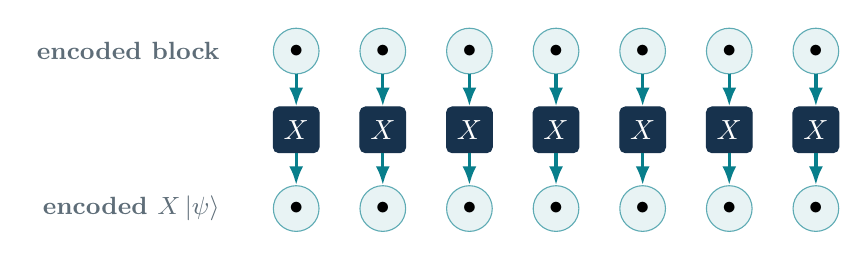
\begin{tikzpicture}[
      >={Latex[length=2.4mm]},
      flow/.style={->,very thick,draw=QFETeal},
      qubit/.style={draw=QFETeal!65,fill=QFEPale,circle,minimum size=0.58cm},
      gate/.style={draw=QFEInk,fill=QFEInk,rounded corners=2pt,
        text=white,minimum size=0.58cm,font=\bfseries}
    ]
    \foreach \x/\name in {-3.3/a1,-2.2/a2,-1.1/a3,0/a4,1.1/a5,2.2/a6,3.3/a7} {
      \node[qubit] (\name) at (\x,1.00) {$\bullet$};
      \node[gate] (g\name) at (\x,0.00) {$X$};
      \node[qubit] (b\name) at (\x,-1.00) {$\bullet$};
      \draw[flow] (\name) -- (g\name);
      \draw[flow] (g\name) -- (b\name);
    }
    \node[font=\small\bfseries,text=QFEMuted,anchor=east] at (-4.15,1.00)
      {encoded block};
    \node[font=\small\bfseries,text=QFEMuted,anchor=east] at (-4.15,-1.00)
      {encoded $X\ket\psi$};
  \end{tikzpicture}

  \vspace{0.25em}
  {\large
  $\displaystyle
    X^{\otimes n}\,\mathsf{QEnc}\ket\psi
      =\mathsf{QEnc}\,X\ket\psi.$\par}

  \vspace{0.55em}
  \takeaway{Apply the same small operation at each coordinate:
    \textbf{local damage stays local}.}

  \note{
    \footnotesize
    \begin{itemize}
      \item $X_L=X^{\otimes n}$ is an intuitive example for the Steane-family code used as a concrete option in the manuscript; it is not a statement about every quantum code.
      \item More generally, a directly supported logical operation $g$ is represented by coordinate operations $g^{(1)},\ldots,g^{(n)}$, which need not all be identical.
      \item Not every operation is available this way. The later magic-state slide explains how the remaining operation is supplied as a preprocessed resource.
      \item This coordinatewise structure is why the construction can check one physical coordinate at a time.
    \end{itemize}
  }
\end{frame}

\begin{frame}{Quantum Authentication: Detect Tampering}
  \centering
  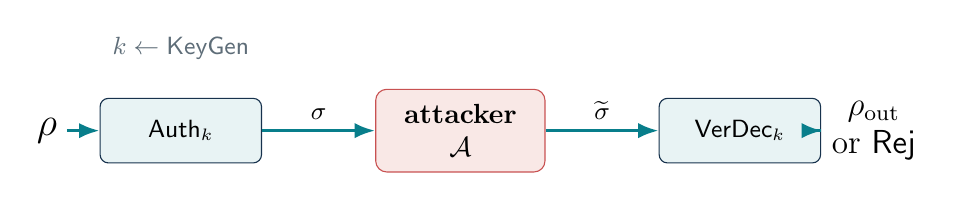
\begin{tikzpicture}[
      >={Latex[length=2.6mm]},
      flow/.style={->,very thick,draw=QFETeal},
      process/.style={draw=QFEInk,fill=QFEFog,rounded corners=3pt,
        minimum width=2.05cm,minimum height=0.82cm,align=center,font=\small\bfseries},
      attacker/.style={draw=QFECoral,fill=QFECoralPale,rounded corners=4pt,
        minimum width=2.15cm,minimum height=1.05cm,align=center,font=\bfseries}
    ]
    \node[font=\Large] (in) at (-5.25,0) {$\rho$};
    \node[process,fill=QFEPale] (auth) at (-3.55,0) {$\mathsf{Auth}_k$};
    \node[attacker] (adv) at (0,0) {attacker\\$\mathcal A$};
    \node[process,fill=QFEPale] (ver) at (3.55,0) {$\mathsf{VerDec}_k$};
    \node[font=\large,align=center] (out) at (5.25,0)
      {$\rho_{\mathrm{out}}$\\or $\rejlabel$};

    \draw[flow] (in) -- (auth);
    \draw[flow] (auth) -- node[above,font=\small] {$\sigma$} (adv);
    \draw[flow] (adv) -- node[above,font=\small] {$\widetilde\sigma$} (ver);
    \draw[flow] (ver) -- (out);
    \node[font=\small\bfseries,text=QFEMuted] at (-3.55,1.05)
      {$k\leftarrow\mathsf{KeyGen}$};
  \end{tikzpicture}

  \vspace{0.9em}
  \begin{alertblock}{Security game}
    \centering
    $\displaystyle
      \text{accept}\quad\Longrightarrow\quad
      \rho_{\mathrm{out}}\approx\rho.$
  \end{alertblock}

  \vspace{-0.15em}
  \takeaway{An attacker may force rejection, but cannot \textbf{change the state
    and still be accepted}.}

  \note{
    \footnotesize
    \begin{itemize}
      \item This is the integrity game. A full definition preserves entanglement with an external reference system.
      \item The attacker can always destroy the authenticated register and force rejection. Authentication prevents an undetected change.
      \item The authenticating key also commonly hides the plaintext, but privacy is not the conceptual point of this slide.
      \item Transition: the trap code is a concrete way to implement this game.
    \end{itemize}
  }
\end{frame}

\begin{frame}{The Trap Code: Hide Data Among Tests}
  \small
  \centering
  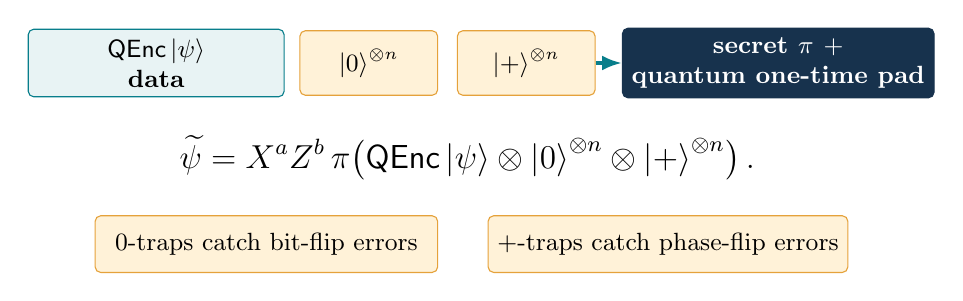
\begin{tikzpicture}[
      >={Latex[length=2.5mm]},
      flow/.style={->,very thick,draw=QFETeal},
      block/.style={draw,rounded corners=2pt,minimum height=0.82cm,
        align=center,font=\small\bfseries}
    ]
    \node[block,draw=QFETeal,fill=QFEPale,minimum width=3.25cm] (data) at (-3.95,0.85)
      {$\mathsf{QEnc}\ket\psi$\\data};
    \node[block,draw=QFEGold,fill=QFEGoldPale,minimum width=1.75cm] (zero) at (-1.25,0.85)
      {$\ket0^{\otimes n}$};
    \node[block,draw=QFEGold,fill=QFEGoldPale,minimum width=1.75cm] (plus) at (0.75,0.85)
      {$\ket+^{\otimes n}$};
    \node[block,draw=QFEInk,fill=QFEInk,text=white,minimum width=2.65cm] (hide) at (3.95,0.85)
      {secret $\pi$ $+$\\quantum one-time pad};
    \draw[flow] (plus.east) -- (hide.west);

    \node[font=\large] at (0,-0.35)
      {$\displaystyle
        \widetilde\psi=X^aZ^b\,\pi\!\left(
          \mathsf{QEnc}\ket\psi\otimes\ket0^{\otimes n}
          \otimes\ket+^{\otimes n}\right).$};

    \node[draw=QFEGold,fill=QFEGoldPale,rounded corners=2pt,
      minimum width=4.35cm,minimum height=0.72cm,font=\small]
      at (-2.55,-1.45) {$0$-traps catch bit-flip errors};
    \node[draw=QFEGold,fill=QFEGoldPale,rounded corners=2pt,
      minimum width=4.35cm,minimum height=0.72cm,font=\small]
      at (2.55,-1.45) {$+$-traps catch phase-flip errors};
  \end{tikzpicture}

  \vspace{0.15em}
  \takeaway{Undo the pad and permutation, test every trap, then decode the data.}

  \vspace{0.1em}
  {\small\color{QFECoral}\textbf{Our protocol:} store QEC $+$ a hidden pad;
    add fresh tests at every gate.\par}

  \note{
    \scriptsize
    \begin{itemize}
      \item The standard trap-code blueprint appends computational-basis and Hadamard-basis test registers, secretly permutes all three blocks, then applies a quantum one-time pad.
      \item Undo the pad and permutation; measure $0$-traps in the computational basis and $+$-traps in the Hadamard basis; only decode if all tests pass.
      \item More precisely, $0$-traps detect $X/Y$ components and $+$-traps detect $Z/Y$ components.
      \item The red footer is important: this manuscript does not keep a persistent standard trap-code ciphertext at the TTP. It inserts fresh tests in every checked operation.
    \end{itemize}
  }
\end{frame}

\begin{frame}{VQFHE: Compute, Then Verify}
  \centering
  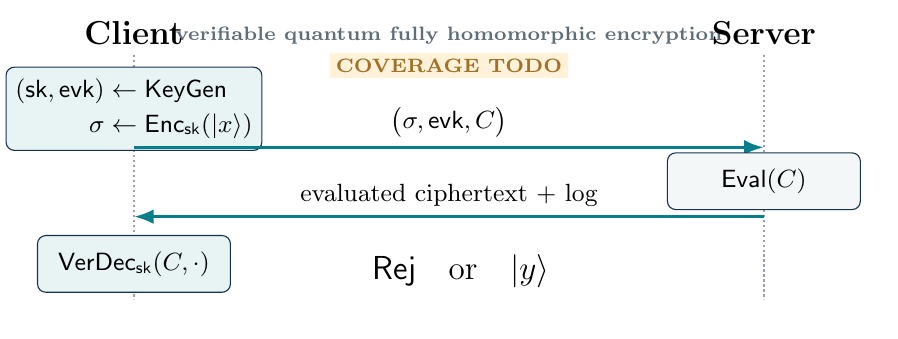
\begin{tikzpicture}[
      >={Latex[length=2.5mm]},
      lane/.style={densely dotted,thick,draw=QFEMuted!65},
      qmsg/.style={->,very thick,draw=QFETeal},
      process/.style={draw=QFEInk,fill=QFEFog,rounded corners=3pt,
        minimum width=2.45cm,minimum height=0.72cm,align=center,font=\small\bfseries}
    ]
    \path[use as bounding box] (-5.35,-1.75) rectangle (5.35,1.85);
    \node[font=\scriptsize\bfseries,text=QFEMuted] at (0,1.75)
      {verifiable quantum fully homomorphic encryption};
    \node[fill=QFEGoldPale,inner sep=2pt,
      font=\scriptsize\bfseries,text=QFEGold!70!black] at (0,1.37)
      {COVERAGE TODO};
    \node[font=\large\bfseries] at (-4.00,1.78) {Client};
    \node[font=\large\bfseries] at (4.00,1.78) {Server};
    \draw[lane] (-4.00,1.50) -- (-4.00,-1.60);
    \draw[lane] (4.00,1.50) -- (4.00,-1.60);

    \node[process,fill=QFEPale] at (-4.00,0.82)
      {$\begin{aligned}(\mathsf{sk},\mathsf{evk})&\leftarrow\mathsf{KeyGen}\\[-0.15em]
        \sigma&\leftarrow\mathsf{Enc}_{\mathsf{sk}}(\ket x)
      \end{aligned}$};
    \draw[qmsg] (-4.00,0.33) -- (4.00,0.33)
      node[midway,above=2pt,font=\small,fill=white,inner sep=1pt]
      {$\bigl(\sigma,\mathsf{evk},C\bigr)$};
    \node[process] at (4.00,-0.10) {$\mathsf{Eval}(C)$};
    \draw[qmsg] (4.00,-0.55) -- (-4.00,-0.55)
      node[midway,above=2pt,font=\small,fill=white,inner sep=1pt]
      {evaluated ciphertext $+$ log};
    \node[process,fill=QFEPale] at (-4.00,-1.15)
      {$\mathsf{VerDec}_{\mathsf{sk}}(C,\cdot)$};
    \node[font=\large] at (0.15,-1.24)
      {$\rejlabel$\quad or\quad $\ket y$};
  \end{tikzpicture}

  \vspace{0em}
  {\small
    \textcolor{QFETeal}{\textbf{Correctness:}}
    $\ket y=C\ket x$
    \qquad
    \textcolor{QFECoral}{\textbf{Verifiability:}}
    accept $\Rightarrow$ correct output.
    \par}

  \vspace{0em}
  \takeaway{Bob evaluates Alice's money verifier without receiving unprotected
    money. \textbf{Custody and incremental checks} make this asset-preserving.}

  \note{
    \scriptsize
    \begin{itemize}
      \item Use the symmetric-key interface of Alagic--Dulek--Schaffner--Speelman: secret key plus quantum evaluation material. Public-key variants can add a public key.
      \item A formal return contains an evaluated ciphertext and log, not a plaintext $\ket{\widetilde y}$.
      \item $\ket y=C\ket x$ is a pure/unitary cartoon. Generally, honest output is $\rho_{\mathrm{out}}\approx\Phi_C(\rho)$, including a reference system.
      \item A malicious server may always force rejection. Generic VQFHE alone does not restore a consumed unique input.
      \item The extra asset-preserving ingredients are TTP custody, an immediate check after each delegated step, and QEC repair.
      \item Reference: \cite{alagic-et-al-vqfhe}.
    \end{itemize}
  }
\end{frame}

\begin{frame}{Homomorphic Evaluation: Act Without Finding the Data}
  \centering
  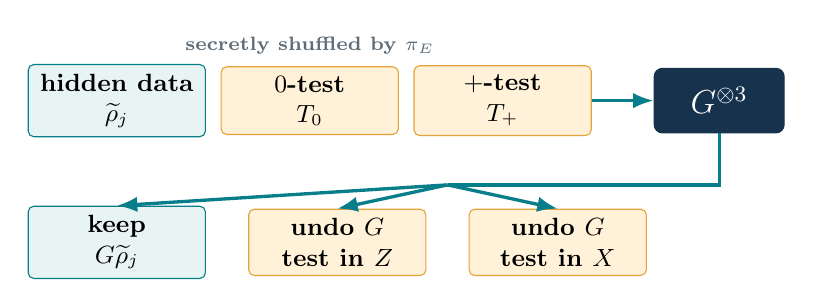
\begin{tikzpicture}[
      >={Latex[length=2.6mm]},
      flow/.style={->,very thick,draw=QFETeal},
      item/.style={draw,rounded corners=2pt,minimum width=2.25cm,
        minimum height=0.82cm,align=center,font=\small\bfseries}
    ]
    \node[item,draw=QFETeal,fill=QFEPale] (d1) at (-4.00,0.85)
      {hidden data\\$\widetilde\rho_j$};
    \node[item,draw=QFEGold,fill=QFEGoldPale] (z1) at (-1.55,0.85)
      {$0$-test\\$T_0$};
    \node[item,draw=QFEGold,fill=QFEGoldPale] (p1) at (0.90,0.85)
      {$+$-test\\$T_+$};
    \node[draw=QFEInk,fill=QFEInk,text=white,rounded corners=3pt,
      minimum width=1.65cm,minimum height=0.82cm,font=\large\bfseries]
      (gate) at (3.65,0.85) {$G^{\otimes3}$};
    \draw[flow] (p1) -- (gate);
    \node[font=\scriptsize\bfseries,text=QFEMuted] at (-1.55,1.55)
      {secretly shuffled by $\pi_E$};

    \node[item,draw=QFETeal,fill=QFEPale] (d2) at (-4.00,-0.95)
      {keep\\$G\widetilde\rho_j$};
    \node[item,draw=QFEGold,fill=QFEGoldPale] (z2) at (-1.20,-0.95)
      {undo $G$\\test in $Z$};
    \node[item,draw=QFEGold,fill=QFEGoldPale] (p2) at (1.60,-0.95)
      {undo $G$\\test in $X$};
    \coordinate (split) at (0.20,-0.22);
    \draw[very thick,draw=QFETeal] (gate.south) |- (split);
    \draw[flow] (split) -- (d2.north);
    \draw[flow] (split) -- (z2.north);
    \draw[flow] (split) -- (p2.north);
  \end{tikzpicture}

  \vspace{0.25em}
  {\large
    $\displaystyle
      \pi_E(\widetilde\rho_j,T_0,T_+)
      \xrightarrow{\quad G^{\otimes3}\quad}
      \pi_E(G\widetilde\rho_j,GT_0,GT_+).$\par}

  \vspace{0.65em}
  \takeaway{The evaluator cannot locate the data, so it must treat the data and
    both tests \textbf{in exactly the same way}.}

  \note{
    \footnotesize
    \begin{itemize}
      \item This is the fresh-trap variant used by the manuscript, not a claim that the at-rest ciphertext is a standard trap-code ciphertext.
      \item Pads and rerandomization are suppressed in the visible formula. The actual evaluator also applies a fresh Pauli rerandomizer.
      \item $G$ denotes a directly supported physical coordinate operation. The TTP prepares the corresponding expected output tests in advance.
      \item After unshuffling, keep the transformed data. Pair returned tests with fresh known tests so that a dishonest checker can also be detected.
      \item Transition directly to Construction II: the next diagram expands this single algebraic operation into its four-message interactive check.
    \end{itemize}
  }
\end{frame}

\begin{frame}[shrink=4]{Construction I: Input Encoding}
  \small
  \centering
  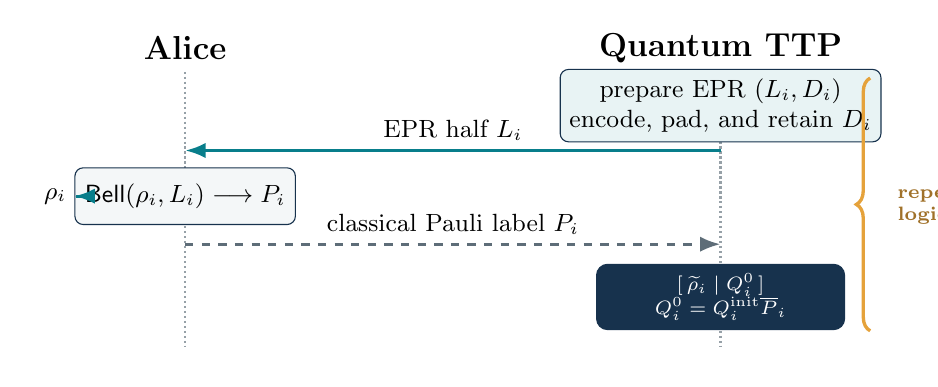
\begin{tikzpicture}[
      >={Latex[length=2.6mm]},
      lane/.style={densely dotted,thick,draw=QFEMuted!65},
      qmsg/.style={->,very thick,draw=QFETeal},
      cmsg/.style={->,very thick,dashed,draw=QFEMuted},
      action/.style={draw=QFEInk,fill=QFEFog,rounded corners=3pt,
        minimum width=3.15cm,minimum height=0.72cm,align=center,font=\small},
      vault/.style={draw=QFEInk,fill=QFEInk,rounded corners=4pt,
        minimum width=3.15cm,minimum height=0.82cm,align=center,text=white,font=\scriptsize}
    ]
    \path[use as bounding box] (-5.55,-2.08) rectangle (5.65,2.12);
    \node[font=\large\bfseries] at (-3.55,1.86) {Alice};
    \node[font=\large\bfseries] at (3.25,1.86) {Quantum TTP};
    \draw[lane] (-3.55,1.56) -- (-3.55,-1.92);
    \draw[lane] (3.25,1.56) -- (3.25,-1.92);

    \node[action,fill=QFEPale] (prep) at (3.25,1.13)
      {prepare EPR $(L_i,D_i)$\\encode, pad, and retain $D_i$};
    \draw[qmsg] (3.25,0.56) -- (-3.55,0.56)
      node[midway,above=2pt,font=\small,fill=white,inner sep=1pt]
      {EPR half $L_i$};
    \node[action,minimum width=2.80cm] (bell) at (-3.55,-0.02)
      {$\mathsf{Bell}(\rho_i,L_i)\longrightarrow P_i$};
    \node[font=\small] (input) at (-5.20,-0.02) {$\rho_i$};
    \draw[qmsg] (input.east) -- (bell.west);
    \draw[cmsg] (-3.55,-0.63) -- (3.25,-0.63)
      node[midway,above=2pt,font=\small,fill=white,inner sep=1pt]
      {classical Pauli label $P_i$};
    \node[vault] (vault) at (3.25,-1.30)
      {$[\,\widetilde\rho_i\mid Q_i^0\,]$\\[-0.1em]
       $Q_i^0=Q_i^{\mathrm{init}}\overline P_i$};

    \draw[decorate,decoration={brace,mirror,amplitude=5pt},very thick,draw=QFEGold]
      (5.15,1.48) -- (5.15,-1.73)
      node[midway,right=6pt,text=QFEGold!70!black,font=\scriptsize\bfseries,align=left]
      {repeat for each\\logical qubit $i$};
  \end{tikzpicture}

  \vspace{-0.25em}
  \begin{exampleblock}{State now in custody}
    \centering
    $\displaystyle
      \widetilde\rho
      =Q^0\,\mathsf{QEnc}(\rho)\,(Q^0)^\dagger.$
  \end{exampleblock}

  \vspace{-0.25em}
  \takeaway{No register carrying $\rho$ travels Alice $\to$ TTP: teleportation
    puts the state into the \textbf{already encoded and padded} half.}

  \note{
    \footnotesize
    \begin{itemize}
      \item The manuscript calls this input commitment; ``teleport into custody'' is clearer for the talk. It is not a bit-commitment primitive.
      \item Operationally, the TTP ends with a fixed encrypted codeword that Alice can no longer modify.
      \item The stored state is a Pauli-padded QECC codeword, not a persistent trap-code ciphertext. Integrity comes from the fresh trap checks on the next slide.
      \item Encoded EPR resources can be prepared offline. Online, the TTP routes $L_i$ and updates a classical Pauli key after receiving $P_i$.
      \item Teleportation preserves entanglement with an external reference system.
    \end{itemize}
  }
\end{frame}

\begin{frame}{Construction II: Gate Evaluation}
  \centering
  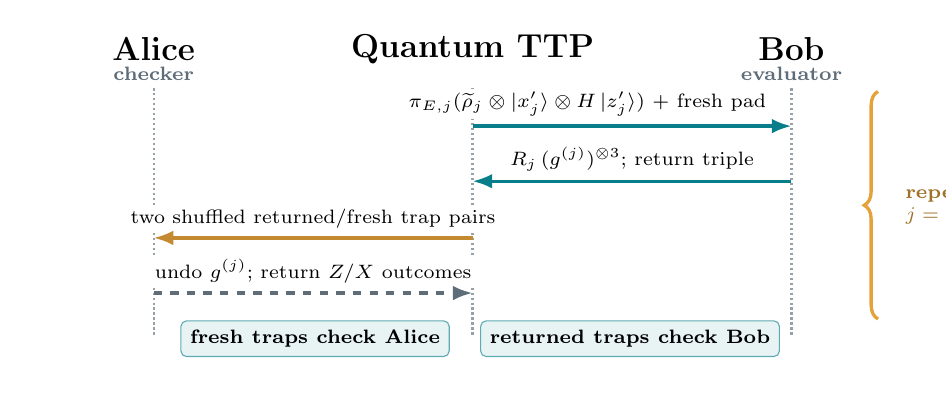
\begin{tikzpicture}[
      >={Latex[length=2.5mm]},
      lane/.style={densely dotted,thick,draw=QFEMuted!65},
      qmsg/.style={->,very thick,draw=QFETeal},
      trapmsg/.style={->,very thick,draw=QFEGold!85!black},
      cmsg/.style={->,very thick,dashed,draw=QFEMuted}
    ]
    \path[use as bounding box] (-5.65,-2.15) rectangle (5.65,2.15);
    \node[font=\large\bfseries] at (-4.05,1.88) {Alice};
    \node[font=\scriptsize\bfseries,text=QFEMuted] at (-4.05,1.57) {checker};
    \node[font=\large\bfseries] at (0,1.88) {Quantum TTP};
    \node[font=\large\bfseries] at (4.05,1.88) {Bob};
    \node[font=\scriptsize\bfseries,text=QFEMuted] at (4.05,1.57) {evaluator};
    \draw[lane] (-4.05,1.38) -- (-4.05,-1.78);
    \draw[lane] (0,1.38) -- (0,-1.78);
    \draw[lane] (4.05,1.38) -- (4.05,-1.78);

    \draw[qmsg] (0,0.90) -- (4.05,0.90)
      node[pos=0.36,above=2pt,font=\scriptsize,fill=white,inner sep=1pt]
      {$\pi_{E,j}(\widetilde\rho_j\otimes\ket{x'_j}\otimes H\ket{z'_j})$ $+$ fresh pad};
    \draw[qmsg] (4.05,0.20) -- (0,0.20)
      node[midway,above=2pt,font=\scriptsize,fill=white,inner sep=1pt]
      {$R_j\,(g^{(j)})^{\otimes3}$; return triple};
    \draw[trapmsg] (0,-0.52) -- (-4.05,-0.52)
      node[midway,above=2pt,font=\scriptsize,fill=white,inner sep=1pt]
      {two shuffled returned/fresh trap pairs};
    \draw[cmsg] (-4.05,-1.22) -- (0,-1.22)
      node[midway,above=2pt,font=\scriptsize,fill=white,inner sep=1pt]
      {undo $g^{(j)}$; return $Z/X$ outcomes};

    \draw[decorate,decoration={brace,mirror,amplitude=5pt},very thick,draw=QFEGold]
      (5.15,1.34) -- (5.15,-1.55)
      node[midway,right=6pt,text=QFEGold!70!black,font=\scriptsize\bfseries,align=left]
      {repeat\\$j=1,\ldots,\ell_{\mathrm{code}}$};

    \node[draw=QFETeal!65,fill=QFEPale,rounded corners=2pt,
      font=\scriptsize\bfseries,align=center,minimum width=3.1cm]
      at (-2.00,-1.80) {fresh traps check Alice};
    \node[draw=QFETeal!65,fill=QFEPale,rounded corners=2pt,
      font=\scriptsize\bfseries,align=center,minimum width=3.1cm]
      at (2.00,-1.80) {returned traps check Bob};
  \end{tikzpicture}

  \vspace{-0.05em}
  \takeaway{Keep the transformed data and update its Pauli key only after the
    checks. Each coordinate hides \textbf{one data register among two traps}.}

  \note{
    \scriptsize
    \begin{itemize}
      \item The mnemonic $\mathsf{OTP}(\ket{\psi_j}\ket0\ket+)$ is right at a high level. The exact call also uses a secret permutation, independent trap pads, and Pauli rerandomization.
      \item Bob applies $(g^{(j)})^{\otimes3}$ because he cannot tell data, $0$-trap, and $+$-trap apart.
      \item Alice receives returned traps mixed with fresh known gate-output traps. This lets the TTP check both roles.
      \item The active manuscript repeats over $j\in[\ell_{\mathrm{code}}]$, not $j\in[3\lambda]$. There are three evaluator registers per call, hence $3\ell_{\mathrm{code}}$ registers over the encoded gate.
      \item After enough detected inconsistencies, replace the evaluator. The QEC is intended to absorb the bounded number of corrupted coordinates before replacement.
      \item Avoid overcommitting to the exact culprit-attribution logic on this slide; that portion of the active algorithm is still being reconciled.
    \end{itemize}
  }
\end{frame}

\begin{frame}{Construction III: Circuit Evaluation}
  \centering
  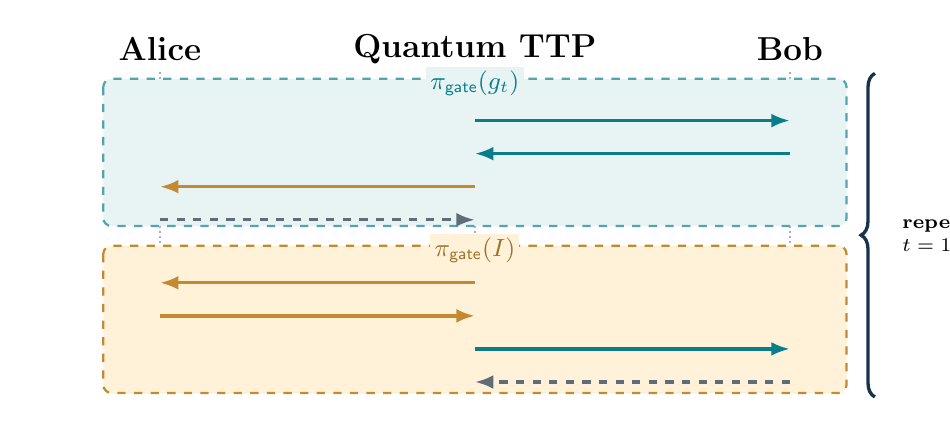
\begin{tikzpicture}[
      >={Latex[length=2.35mm]},
      lane/.style={densely dotted,thick,draw=QFEMuted!55},
      qmsg/.style={->,very thick,draw=QFETeal},
      trapmsg/.style={->,very thick,draw=QFEGold!85!black},
      cmsg/.style={->,very thick,dashed,draw=QFEMuted}
    ]
    \path[use as bounding box] (-5.68,-2.47) rectangle (5.68,2.38);
    \node[font=\large\bfseries] at (-4.00,2.11) {Alice};
    \node[font=\large\bfseries] at (0,2.11) {Quantum TTP};
    \node[font=\large\bfseries] at (4.00,2.11) {Bob};
    \draw[lane] (-4,1.82) -- (-4,-2.25);
    \draw[lane] (0,1.82) -- (0,-2.25);
    \draw[lane] (4,1.82) -- (4,-2.25);

    \draw[draw=QFETeal!70,fill=QFEPale,rounded corners=3pt,dashed,thick]
      (-4.72,1.73) rectangle (4.72,-0.14);
    \node[fill=QFEPale,inner sep=1.5pt,font=\small\bfseries,text=QFETeal]
      at (0,1.67) {$\pi_{\mathsf{gate}}(g_t)$};
    \draw[qmsg] (0,1.20) -- (4,1.20);
    \draw[qmsg] (4,0.78) -- (0,0.78);
    \draw[trapmsg] (0,0.36) -- (-4,0.36);
    \draw[cmsg] (-4,-0.06) -- (0,-0.06);

    \draw[draw=QFEGold!85!black,fill=QFEGoldPale,rounded corners=3pt,dashed,thick]
      (-4.72,-0.39) rectangle (4.72,-2.26);
    \node[fill=QFEGoldPale,inner sep=1.5pt,font=\small\bfseries,text=QFEGold!70!black]
      at (0,-0.45) {$\pi_{\mathsf{gate}}(I)$};
    \draw[trapmsg] (0,-0.86) -- (-4,-0.86);
    \draw[trapmsg] (-4,-1.28) -- (0,-1.28);
    \draw[qmsg] (0,-1.70) -- (4,-1.70);
    \draw[cmsg] (4,-2.12) -- (0,-2.12);

    \draw[decorate,decoration={brace,mirror,amplitude=5pt},very thick,draw=QFEInk]
      (5.08,1.80) -- (5.08,-2.31)
      node[midway,right=6pt,font=\scriptsize\bfseries,align=left]
      {repeat for\\$t=1,\ldots,T$};
  \end{tikzpicture}

  \vspace{-0.15em}
  \takeaway{For each \textbf{circuit step}: one party evaluates and the other
    checks; then reverse roles and refresh.}

  \note{
    \scriptsize
    \begin{itemize}
      \item For Alice's asset, Alice is the sender and Bob the verifier. Bob evaluates the actual gate and Alice checks; the identity pass reverses their roles.
      \item Show all eight arrows even if the labels are abbreviated; the repeated geometry is the point.
      \item A circuit is not eight messages total: the pair repeats for every directly supported instruction and each gate call repeats over every physical coordinate.
      \item The identity pass makes both parties serve as evaluator and refreshes the hidden state before the next instruction.
      \item Measurement instructions use a separate trap-checked primitive. Other gate and measurement details in the active rewrite are less polished, so keep the visible claim to one generic circuit step.
      \item This is a candidate construction. The load-bearing coherent-attack security argument is still being finalized; do not present it as a finished theorem.
    \end{itemize}
  }
\end{frame}

\begin{frame}{Preprocessing: The Quantum Resource Bank}
  \small
  \begin{columns}[T,onlytextwidth]
    \column{0.315\textwidth}
      \begin{exampleblock}{Input custody}
        \centering
        encoded, padded\\
        EPR halves

        \medskip
        \faArchive\quad $\widetilde D_i$
      \end{exampleblock}

    \column{0.315\textwidth}
      \begin{exampleblock}{Workspace}
        \centering
        encoded, padded\\
        $\ket0$ and $\ket T$ blocks

        \medskip
        $\ket T:=T\ket+$
      \end{exampleblock}

    \column{0.315\textwidth}
      \begin{exampleblock}{Checks}
        \centering
        fresh $0/+$ gate traps\\
        and measurement traps

        \medskip
        \faLock\quad hidden tests
      \end{exampleblock}
  \end{columns}

  \vspace{0.25em}
  \begin{columns}[T,onlytextwidth]
    \column{0.47\textwidth}
      \begin{block}{Classical ledger}
        \centering
        Pauli keys, secret permutations,\\
        expected trap outcomes
      \end{block}

    \column{0.47\textwidth}
      \begin{alertblock}{One-use quantum fuel}
        \centering
        Consuming one $\ket T=T\ket+$ state in a checked gadget
        implements a $T$ gate.
      \end{alertblock}
  \end{columns}

  \vspace{-0.15em}
  \takeaway{Once the bank is stocked, the TTP's online job is
    \textbf{storage + routing/SWAP}, with classical checks and key updates.}

  \note{
    \scriptsize
    \begin{itemize}
      \item This slide collects the quantum material prepared before the exchange begins.
      \item Input resources are encoded, Pauli-padded halves of EPR pairs. Alice teleports her state into the retained half during Construction I.
      \item Workspace includes encoded padded $\ket0$ ancillas and encoded padded $\ket T$ magic states. A standard injection consumes $\ket T$ using an entangling operation, a measurement, and outcome-controlled corrections.
      \item Check material includes fresh gate-dependent $0$- and $+$-trap bundles, plus the traps needed by measurement calls. For an adaptive circuit, the draft preprocesses candidate bundles for every supported operation at a slot and discards the unused candidates.
      \item The trusted party also retains a classical ledger of pads, permutations, and expected outcomes.
      \item This is the intended resource boundary of the candidate construction; exact counts will change as the active proof and gadgets are finalized.
    \end{itemize}
  }
\end{frame}

\begin{frame}{Construction IV: Full Exchange}
  \centering
  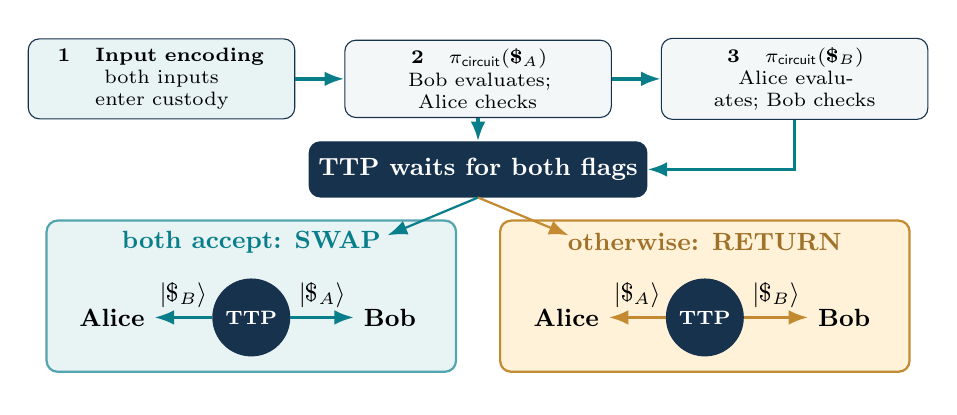
\begin{tikzpicture}[
      >={Latex[length=2.5mm]},
      flow/.style={->,very thick,draw=QFETeal},
      stage/.style={draw=QFEInk,fill=QFEFog,rounded corners=4pt,
        text width=3.15cm,minimum height=0.98cm,align=center,font=\scriptsize},
      decision/.style={draw=QFEInk,fill=QFEInk,rounded corners=4pt,
        minimum width=3.45cm,minimum height=0.70cm,text=white,align=center,font=\small\bfseries},
      party/.style={font=\small\bfseries}
    ]
    \path[use as bounding box] (-5.72,-2.36) rectangle (5.72,2.20);
    \node[stage,fill=QFEPale] (encode) at (-4.02,1.55)
      {\textbf{1\quad Input encoding}\\both inputs\\enter custody};
    \node[stage] (verifya) at (0,1.55)
      {\textbf{2\quad $\pi_{\mathsf{circuit}}(\asset{A})$}\\Bob evaluates; Alice checks};
    \node[stage] (verifyb) at (4.02,1.55)
      {\textbf{3\quad $\pi_{\mathsf{circuit}}(\asset{B})$}\\Alice evaluates; Bob checks};
    \draw[flow] (encode) -- (verifya);
    \draw[flow] (verifya) -- (verifyb);

    \node[decision] (decision) at (0,0.40)
      {TTP waits for both flags};
    \draw[flow] (verifya.south) -- (decision.north);
    \draw[flow] (verifyb.south) |- (decision.east);

    \draw[draw=QFETeal!70,fill=QFEPale,rounded corners=4pt,thick]
      (-5.48,-0.25) rectangle (-0.28,-2.17);
    \node[font=\small\bfseries,text=QFETeal] at (-2.88,-0.52)
      {both accept: SWAP};
    \node[party] (as) at (-4.65,-1.48) {Alice};
    \node[draw=QFEInk,fill=QFEInk,circle,text=white,minimum size=0.68cm,font=\scriptsize\bfseries]
      (ts) at (-2.88,-1.48) {TTP};
    \node[party] (bs) at (-1.12,-1.48) {Bob};
    \draw[flow] (ts) -- (as)
      node[midway,above=2pt,font=\small,fill=QFEPale,inner sep=1pt] {$\qasset{B}$};
    \draw[flow] (ts) -- (bs)
      node[midway,above=2pt,font=\small,fill=QFEPale,inner sep=1pt] {$\qasset{A}$};

    \draw[draw=QFEGold!85!black,fill=QFEGoldPale,rounded corners=4pt,thick]
      (0.28,-0.25) rectangle (5.48,-2.17);
    \node[font=\small\bfseries,text=QFEGold!70!black] at (2.88,-0.52)
      {otherwise: RETURN};
    \node[party] (af) at (1.12,-1.48) {Alice};
    \node[draw=QFEInk,fill=QFEInk,circle,text=white,minimum size=0.68cm,font=\scriptsize\bfseries]
      (tf) at (2.88,-1.48) {TTP};
    \node[party] (bf) at (4.65,-1.48) {Bob};
    \draw[->,very thick,draw=QFEGold!85!black] (tf) -- (af)
      node[midway,above=2pt,font=\small,fill=QFEGoldPale,inner sep=1pt] {$\qasset{A}$};
    \draw[->,very thick,draw=QFEGold!85!black] (tf) -- (bf)
      node[midway,above=2pt,font=\small,fill=QFEGoldPale,inner sep=1pt] {$\qasset{B}$};

    \draw[->,thick,draw=QFETeal] (decision.south) -- ++(-1.15,-0.48);
    \draw[->,thick,draw=QFEGold!85!black] (decision.south) -- ++(1.15,-0.48);
  \end{tikzpicture}

  \vspace{-0.15em}
  \takeaway{Preprocess encoded EPR halves and gate-dependent traps. Online,
    the TTP uses \textbf{quantum storage + routing/SWAP}, with classical checks
    and Pauli-key updates.}

  \note{
    \scriptsize
    \begin{itemize}
      \item The two one-sided circuit evaluations leave both processed encrypted assets and their updated Pauli keys at the TTP until both flags are known.
      \item On success the outputs cross. On failure each updated asset returns to its original owner.
      \item Bob runs the public circuit that validates Alice's asset; Alice runs the circuit validating Bob's. The active source has some subscript naming still being cleaned up.
      \item Fairness comes from delayed release: neither party gets the other's unique asset before both checks complete.
      \item Quantum resources used online can be prepared in advance. The TTP's online quantum behavior is intended to reduce to storage, communication, and hidden permutations implemented with routing/SWAP; checks and key updates are classical.
      \item This removes the classical fork from the impossibility proof: the adjudicator now holds irreplaceable quantum custody.
      \item Say ``candidate construction'' while the complete security proof and several circuit-gadget details remain in progress.
    \end{itemize}
  }
\end{frame}

% Bibliography is an unnumbered backup frame rather than part of the ten-frame
% motivation slides, impossibility narrative, and construction sketch above.
\begin{frame}[allowframebreaks,noframenumbering]{References}
  \scriptsize
  \printbibliography[heading=none]
\end{frame}

\end{document}
